% !TeX root = ADP-SG-Tester.tex

\chapter{Comparison of different policies}\label{ch:ComparisonTheory}

This chapter introduces the concepts applied to compare the different policies. \Cref{s:GenData} presents the process of how the evaluation data is generated. \Cref{s:TheoryTtest} explains the theory on statistical testing which policy performs best and \Cref{s:CompWorkEx} finally compares the various policies introduced before on the working example.

\section{Process of generating evaluation data}\label{s:GenData}

In the previous chapter, we introduced various algorithms and solved the problem of how to determine which set of products should be offered given a certain time and given certain capacities of resources remaining. Now, we want to evaluate the trained algorithms. Therefore, we prepare unseen data, which is sometimes also called data based on exogenous information. We set up a total of $K$ sample paths, each determined by its associated customer stream and sales stream. Of the $K$ \emph{customer streams}, each consists of $T$ time periods. So, all customer streams are represented by a matrix $\in \mathbb{R}^{K\times T}$ of uniformly distributed random variables. In the same way, a matrix of random numbers is used for the \emph{sales stream}. These two entities determine the sample paths, are kept fixed in the whole analysis and used for every algorithm.

Every single algorithm now runs for a given setting (possibly the starting capacities or no-purchase preference change among settings) on each of the $K$ scenarios. It starts at $t=0$ with capacity $\boldsymbol{c}^0$. The offerset is determined by the trained algorithm and a sales process is simulated given the current value of the customer stream and sales stream random variables. Then, the time value $t$ is incremented and if a product was sold, the capacity vector is adjusted in accordance with the resources needed. In such a manner, all time periods are evaluated and it is kept track of the offersets offered, products sold, left over capacities and value generated.

We now want to point out some peculiarities of each algorithm.

\begin{itemize}
	\item ES: The exact solution uses a lookup table to explicitly lookup which offerset is optimal for a given state $(t, \boldsymbol{c})$.
	\item CDLP: The choice based deterministic linear program determines at the start, \ie at  $(0, \boldsymbol{c}^0)$, for how many time periods which offersets shal be offered and allows for non integer (continuous) time periods. As we have discrete time periods, we offer a particular offerset for the assigned time periods, rounded to the next integer value. If rounding doesn't lead to an admissable assignment of offersets to time periods\footnote{The sum of rounded assigned time periods is either greater or smaller then the total number of time periods.}, this is adjusted manually and pointed out in the document. Furthermore, as time evolves, some products might not be allowed to be offered any longer (not all resources are available any longer). If such a thing occurs, the affected product is simply removed from the offerset.
	\item API: Given a particular state $(t, \boldsymbol{c})$, the offerset is determined with the associated value of $\boldsymbol{\pi}$.
\end{itemize}

For all examples, we use $K = 5.000$\ and $T$ as specified in the example.

\section{Theory on two sample test}\label{s:TheoryTtest}

The main measure determining the goodness of a policy is the value it generates over the time horizon. But to be confident in the statement that one policy is better then another, we need to apply a statistical test and will introduce general theory on this in the following.

Our goal is to evaluate two different policies. One policy is considered better then another policy if it generally leads to higher total revenues. To put this vague phrasing into a scientifically sound comparison, we use an \emph{approximate two sample test}, which we'll describe here in more detail. This overview and notation is mainly based on Ch. 14.7 of \cite{Bamberg.2011} with extensions as in Ch. 11.3 of \cite{Fahrmeir.2007}.

As elaborate in \Cref{s:GenData}, we have a total of $K$ sample paths. A certain policy applied to one particular sample path will generate a value of $v$, \ie starting at time $t=0$ with capacities $\boldsymbol{c}^0$ and the exogenous information associated with this sample path (customer stream and sales stream), a total value of $v$ is generated. Thus, policy $A$ applied to all sample paths generates the vector of values $\boldsymbol{v}^A \in \mathbb{R}^K$. Accordingly for policy $B$, $\boldsymbol{v}^B$ is determined. As both policies rely on the same exogenous information, the samples are dependent and a \emph{paired samples t-test} has to be used.

Thus, we end up with two observations of size $K$ 

$$v^A_1, \dots, v^A_K \text{  respectively  } v^B_1, \dots, v^B_K~.$$

Let $\bar{\boldsymbol{v}}^A$ and $s_A^2$ resp.\xspace $\bar{\boldsymbol{v}}^B$ and $s_B^2$ be the empirical mean and empirical variance. Furthermore, $\mu^A$ and $\sigma_A^2$ denote the expected value and variance of $v^A_i$, respectively $\mu^B$ and $\sigma_B^2$ denote the expected value and variance of $v^B_i$. To test the hypothesis \enquote{policy $A$ is better then policy $B$}, we use the following null and alternative hypothesis:

$$H_0: \mu^A \leq \mu^B,~~ H_1: \mu^A > \mu^B~.$$

As $\bar{\boldsymbol{v}}^A$ and $\bar{\boldsymbol{v}}^B$ are unbiased estimators of $\mu^A$ and $\mu^B$, the difference $D = \bar{\boldsymbol{v}}^A - \bar{\boldsymbol{v}}^B$ can be used to test the hypothesis. A large value of $D$ represents the data to be in favour of $H_1$. 

As the sample size $K$ satisfies $K > 30$ and the distribution of $v^A_i$ or $v^B_i$ is unknown, it can be derived for the test statistic
$$T = \frac{\bar{\boldsymbol{v}}^A - \bar{\boldsymbol{v}}^B}{\sqrt{\frac{s_A^2 + s_B^2}{K}}} \sim N(0; 1)~.$$

With this knowledge, we can compute the $p$-value according to $p = 1 - \Phi(T)$ with $\Phi(\cdot)$ being the standard normal distribution function. Note: The $p$-value can be seen as evidence against $H_0$. A small $p$-value represents strong evidence against $H_0$ and the null hypothesis should be rejected if the $p$-value is below a significance threshold $\alpha$.

We use $\alpha = 0.05$ to claim one policy being significantly better then another.

\section{Comparison applied to Working example}\label{s:CompWorkEx}

In the following, we apply the previously introduced ways of comparing different policies to our working example. We start of with comparing the values generated, continue with offersets offered, products sold and what capacities remained in the final period, and close with statistical tests on which policy is better then another.

\subsection{Value generated}

A good first overview on the different policies is presented by \Cref{fig-comp-work-val}. \Cref{fig-comp-work-valBox} presents a classic boxplot of the values generated by each policy. It can clearly be seen that ES performs quite well and achieves the overall maximum. Also CDLP performs very well and one cannot tell yet, whether it is significantly worse then ES. For API, we actually used two sets of values for $\boldsymbol{\pi}$, one coming from the last policy iteration (API60) and one from the second last (API59). The alternating effect that has already been observed in the training process, compare \Cref{fig-adp-valueFunc}, can again be seen and actually the $\boldsymbol{\pi}$'s of the second last iteration seem to perform much better, but also fall short behind ES and CDLP. Even more information on the distribution of the generated values by each policy can be found in the violinplot presented in \Cref{fig-comp-work-valVio}. ES and CDLP have more bumps, though certain values are generated with higher likelihood. Both API policies have less bumps, thus the generated values cluster less.

\begin{figure}[!ht]
	\begin{subfigure}[t]{.5\textwidth}
		\centering	
		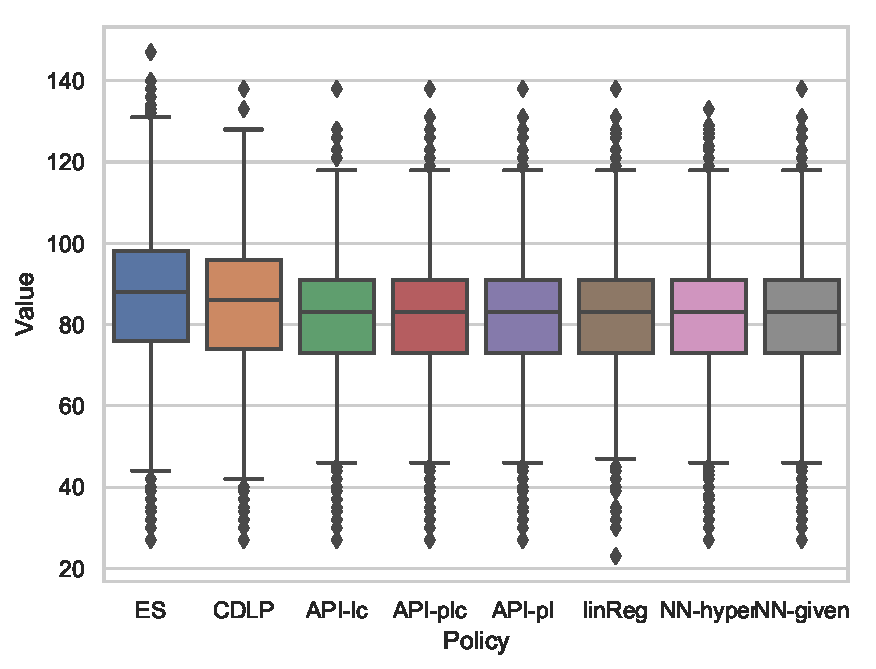
\includegraphics[width=\linewidth]{C:/Users/Stefan/LRZ Sync+Share/Masterarbeit-Klein/Code/Results/exampleStefan-True-ALL-comparison-190923-1732/values-Boxplot.pdf}
		\caption{\label{fig-comp-work-valBox} Boxplot}
	\end{subfigure}%
	\begin{subfigure}[t]{.5\textwidth}
		\centering
		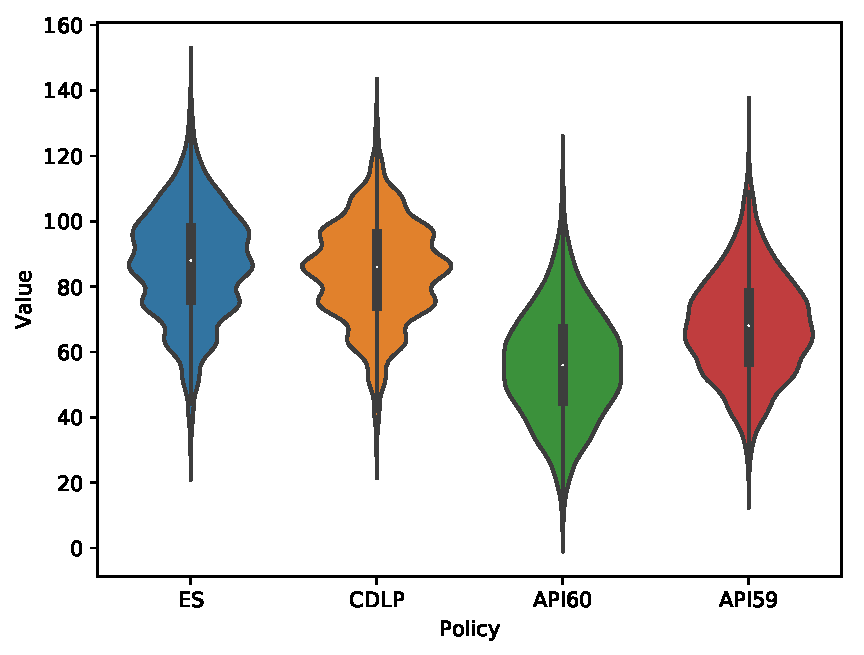
\includegraphics[width=\linewidth]{C:/Users/Stefan/LRZ Sync+Share/Masterarbeit-Klein/Code/Results/exampleStefan-True-ALL-comparison-190923-1732/values-Violinplot.pdf}
		\caption{\label{fig-comp-work-valVio} Violinplot}
	\end{subfigure}
	\caption[Box- and Violinplot for comparison of working example - values.]{\label{fig-comp-work-val}Box- and Violinplot to compare different policies on the working example by their generated values.}
\end{figure}

The previous observations are underlined by the summary statistics presented in \Cref{tb-comp-work-val}. It depicts that indeed $K=5.000$ sample paths are used for evaluation. ES generates the highest mean ($87.11$) and also the highest total revenue ($147$). Interestingly, also its minimum value ($27$) is higher or equal to the minimum value of the other policies. This is a first indicator of ES being indeed the optimal policy.

\begin{table}
	\centering
	\input{"C:/Users/Stefan/LRZ Sync+Share/Masterarbeit-Klein/Code/Results/exampleStefan-True-ALL-comparison-190923-1732/values-Summary.txt"}
	\caption[Summary statistics for comparison of working example - values.]{\label{tb-comp-work-val}Summary statistics to compare different policies on the working example by their generated values.}
\end{table}

\subsection{Offersets offered}



\begin{figure}[!ht]
%	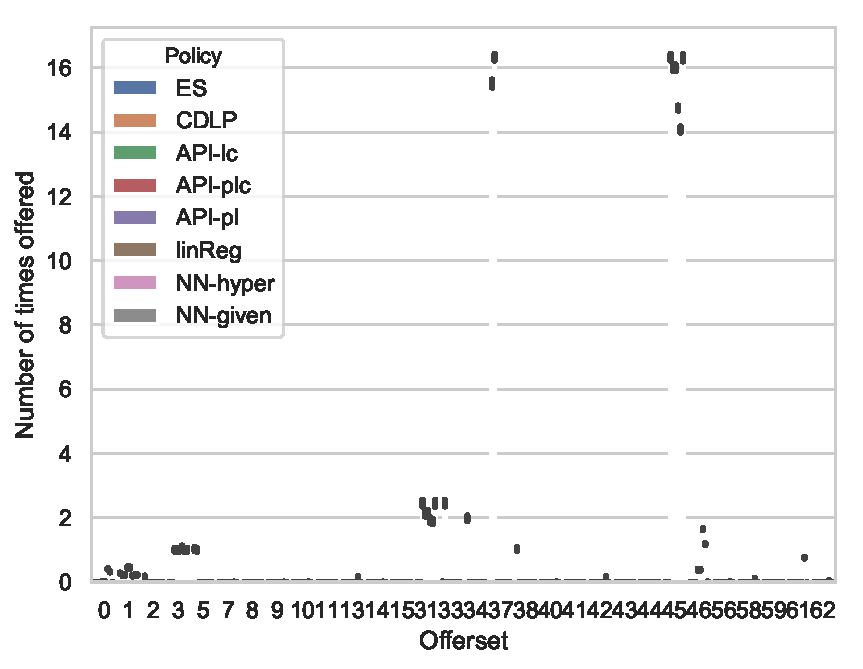
\includegraphics[width=.6\linewidth]{C:/Users/Stefan/LRZ Sync+Share/Masterarbeit-Klein/Code/Results/exampleStefan-True-ALL-comparison-190923-1732/offersets-Barplot.pdf}
%	\quad
%	\scriptsize
%	\input{"C:/Users/Stefan/LRZ Sync+Share/Masterarbeit-Klein/Code/Results/exampleStefan-True-ALL-comparison-190923-1732/offersets-Overview.txt"}%
%
%	\begin{subfigure}[t]{.5\textwidth}
%		\centering
%		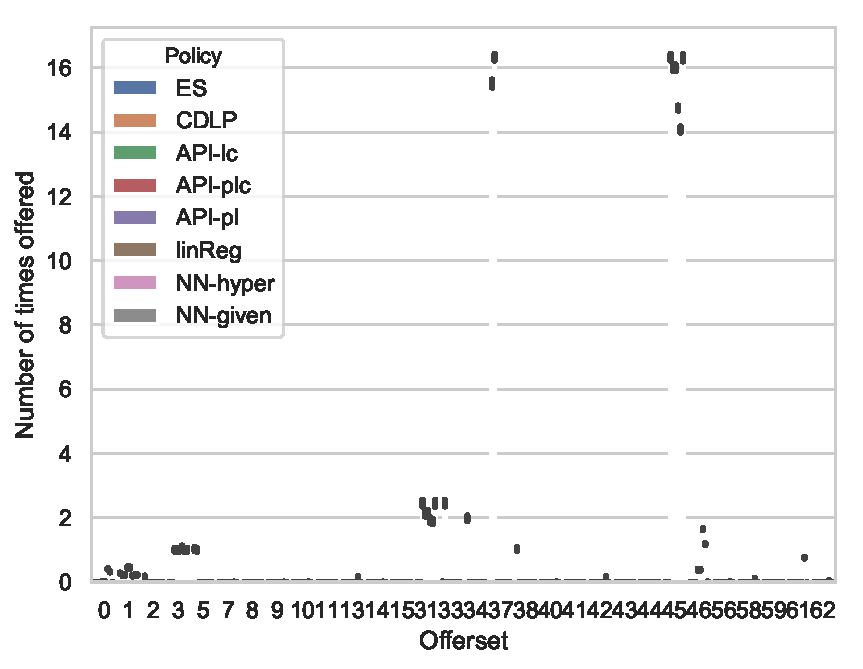
\includegraphics[width=\linewidth]{C:/Users/Stefan/LRZ Sync+Share/Masterarbeit-Klein/Code/Results/exampleStefan-True-ALL-comparison-190923-1732/offersets-Barplot.pdf}
%	\end{subfigure}%
%	\begin{subfigure}[t]{.5\textwidth}
%		\footnotesize
%		\input{"C:/Users/Stefan/LRZ Sync+Share/Masterarbeit-Klein/Code/Results/exampleStefan-True-ALL-comparison-190923-1732/offersets-Overview.txt"}
%	\end{subfigure}%
	\begin{minipage}[t][7cm][t]{.6\textwidth}
		\centering
		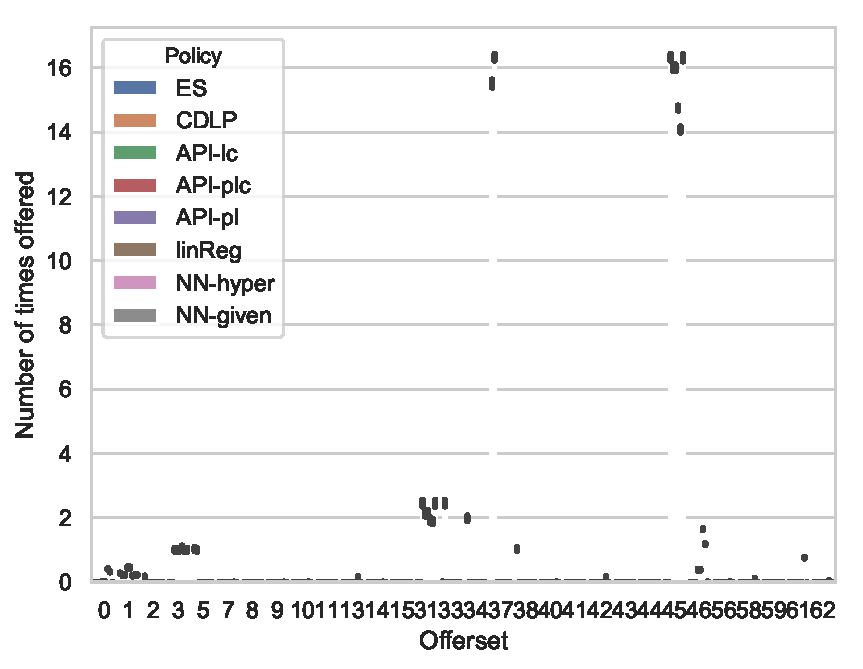
\includegraphics[width=\linewidth]{C:/Users/Stefan/LRZ Sync+Share/Masterarbeit-Klein/Code/Results/exampleStefan-True-ALL-comparison-190923-1732/offersets-Barplot.pdf}
		%		\vfill
	\end{minipage}%
	\quad
	\begin{minipage}[b][7cm][t]{.5\textwidth}
		\vspace*{1cm}
		\scriptsize
		\input{"C:/Users/Stefan/LRZ Sync+Share/Masterarbeit-Klein/Code/Results/exampleStefan-True-ALL-comparison-190923-1732/offersets-Overview.txt"}
		%		\vfill
	\end{minipage}%
	\caption[Barplot for comparison of working example - offersets.]{\label{fig-comp-work-off}Barplot to compare different policies on the working example by their offered products.}
\end{figure}

\subsection{Products sold}

\begin{figure}[!ht]
	\centering	
	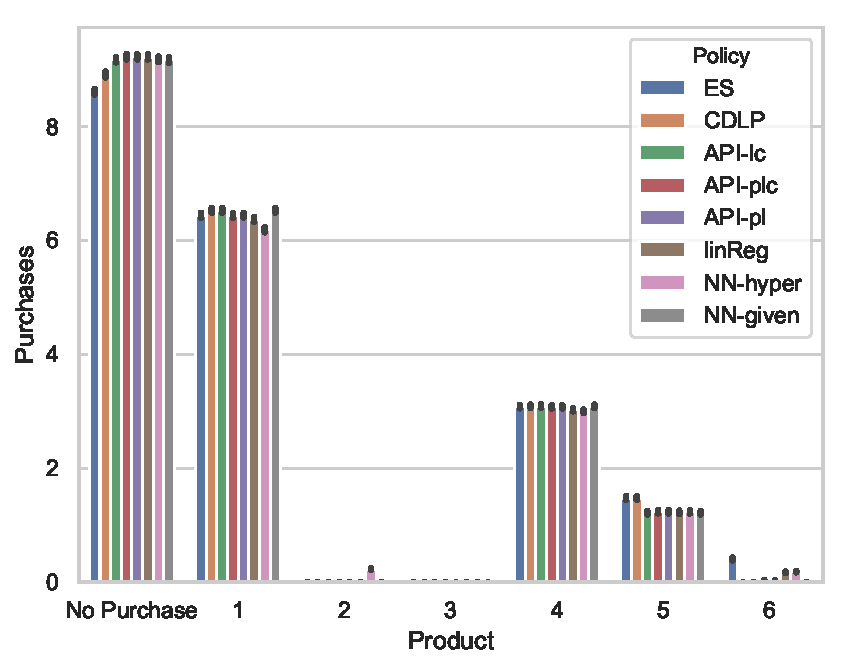
\includegraphics[width=.7\linewidth]{C:/Users/Stefan/LRZ Sync+Share/Masterarbeit-Klein/Code/Results/exampleStefan-True-ALL-comparison-190923-1732/products-Barplot.pdf}
	\caption[Barplot for comparison of working example - products.]{\label{fig-comp-work-prod}Barplot to compare different policies on the working example by their sold products.}
\end{figure}%

\subsection{Capacities remaining}

\begin{figure}[!ht]
	\centering	
	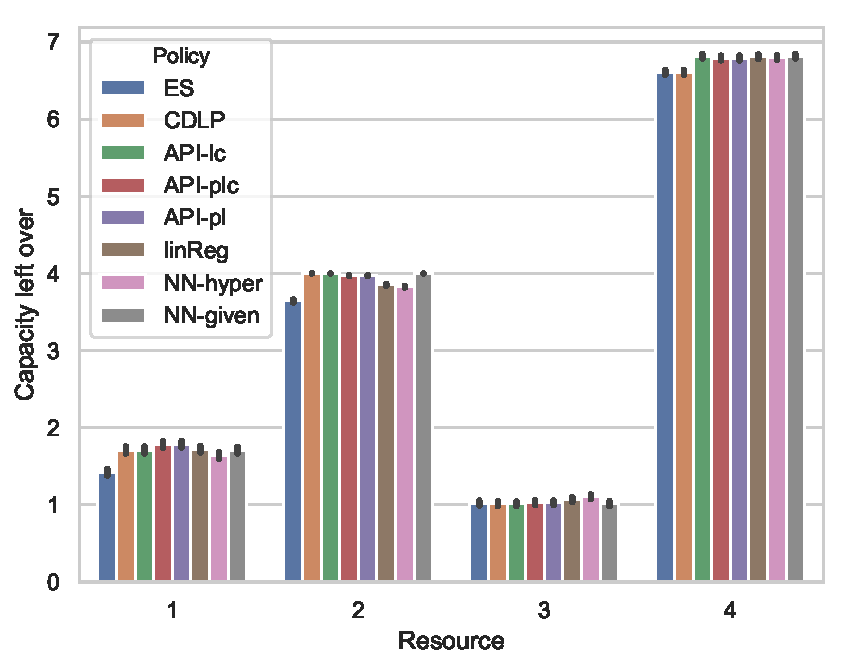
\includegraphics[width=.7\linewidth]{C:/Users/Stefan/LRZ Sync+Share/Masterarbeit-Klein/Code/Results/exampleStefan-True-ALL-comparison-190923-1732/resources-Barplot.pdf}
	\caption[Barplot for comparison of working example - resources.]{\label{fig-comp-work-res}Barplot to compare different policies on the working example by their remaining capacities.}
\end{figure}%


\subsection{Statistical tests}